\chapter{Lien entre les instants de réionisation des galaxies et la masse de leurs halo à l'époque actuelle}
%RELATING THE REIONIZATION TIMES OF GALAXIES TO THEIR PRESENT HALO MASSES

\section{Le projet Cosmic Dawn}
\label{sec:CODAEMMA}

Les simulations présentées jusqu'ici ont toutes une taille de $\left( 8\cdot h^{-1} \mathrm{cMpc} \right)^3$.
Cette taille présente l'avantage de pouvoir réaliser un grand nombre de simulations facilement sans que cela na coûte trop cher en temps de calcul.
Mais il est admit que cette taille est trop faible pour étudier la réionisation dans son ensemble.
Les séries de simulations présentées ont pour vocation de calibrer et d'améliorer notre compréhension une simulation plus ambitieuse que je vais présenter dans ce chapitre.


%Lettre donc partie courte.

Cette partie repose sur une lettre qui s'inscrit dans une stratégie de travail a long terme.
Elle a pour vocation de présenter la simulation "\ac{CoDa} I AMR" ainsi que les premiers résultats obtenus.
Ces résultats utilise deux simulation pour faire le lien entre la période de réionisation et l’époque actuelle.
Je vais présenter les deux simulations utilisées et la façon dont le lien entre les deux est fait.
Cette étude montre que les halos les plus massifs a z=0 sont réionisé plus tôt que le reste de l'Univers.

%Objectif connaitre le Z reio des halo en fonction de leur masse.
%Sur grosse simu donc beaucoup de stats

%\subsection{Présentation de la simulation CODA II EMMA}

\subsection{Présentation des simulations et conditions initiales}

Le projet \ac{CoDa} a pour objectif d'étudier la réionisation du groupe local, et de comprendre si il s'est fait réionisé par  ou si il s'est réionisé de manière autonome.
Pour se faire, un contexte cosmologique suffisamment large est nécessaire pour modéliser l'influence des grandes structures comme Virgo ou Fornax par exemple.
Les conditions initiales ont été générées par la collaboration \ac{CLUES}, avec pour objectif de retrouver dans la simulation, des structures ayant des caractéristiques proches de ce qui est observé dans l'univers local.
On cherchera par exemple à obtenir un couple Andromède - Voie Lacté avec des masses, distances et vitesses relative en accord avec les contraintes actuelles.

Les conditions initiales utilisées ici sont une version basse résolution de celles utilisée par la simulation \ac{CoDa} I \citep{ocvirk_cosmic_2015}.
Cette simulation a été réalisé avec le code RAMSES CUDATON %TODO ref
considère un volume de $\left( 64/h \mathrm{cMpc} \right)^3$ et est échantillonné par $4096^3$ particules de matière noire.
Dans le cas de l'étude présentée ici, cette résolution a été dégradée en $2048^3$, ce qui mène à une résolution en masse $3.4 \cdot 10^6 M_\odot$ et une résolution spatiale de 46 ckpc sur la grille de base, permettant d'explorer une gamme de masse de halos comprise entre $10^8 M_\odot$ et $10^{13}M_\odot$.
La perte d'un niveau de résolution est compensé par l'utilisation de l'\ac{AMR} de EMMA, permettant d’augmenter la résolution spatiale au détriment de la résolution en masse.
L'objectif est de pouvoir faire une comparaison directe entre les deux versions de cette simulation (CoDa I RAMSES CUDATON vs CoDa I AMR) dans un avenir proche.

%différences avec CODA I RAMSES CUDATON et future comparaisons
%8x moins résolue en masse 
%Mais mieux résolue en dx

A partir de ces conditions initiales plusieurs simulations ont été réalisées.
Le première est une simulation de N-corps pur, ne considérant que la matière noire.
Elle a été réalisée avec le code Gadget \citep{springel_cosmological_2005} jusqu'à redshift $z=0$.
Cette première a pour objectif de suivre l'évolution des structures jusqu'à redshift $z=0$.
La seconde est une simulation \ac{RHD} entièrement couplé réalisé avec EMMA.
Elle est focalisée sur l'\ac{EoR} et elle s’arrête donc à redshift $z=6$, une fois l'Univers réionisé.
Cette simulation a été exécutée sur le calculateur TITAN (voir section \ref{sec:titan}) et a utilisée 32768 cœurs \ac{CPU} et 4096 \ac{GPU}.
Les travaux présentés dans la section \ref{sec:etoiles} ont aidés de calibrer correctement la simulation.
Les comparaisons aux contraintes observationnelles de la \ac{SFH} cosmique, de l'évolution de le fraction ionisée et de l'épaisseur optique Thomson sont présentées sur la figure \ref{fig:presCODAEMMA}. 
La concordance est excellente.

La simulation EMMA a pour but d'obtenir une représentation complète de l'époque de réionisation via sa carte de redshift d'ionisation.
L'implémentation du calcul de cette carte à la volée (voir section \ref{sec:zmapcompute}) a permis d'obtenir une excellente résolution temporelle.
Cependant, des difficultés de gestion mémoire ont menés à arrêter le calcul de cette carte à la volée à partir de redshift $z=8$.
Après ce redshift, la carte a été obtenues à l'aide des sorties disques, plus espacées en temps.
Malgré cet incident, la résolution temporelle est au pire de 1.4 Myrs à redshift $z=6$, ce qui est inférieur au temps de vie d'une étoile, et reste donc acceptable.

%TODO génération de la carte de redshift problème de gestion mémoire mix entre carte et sorties

\begin{figure}
        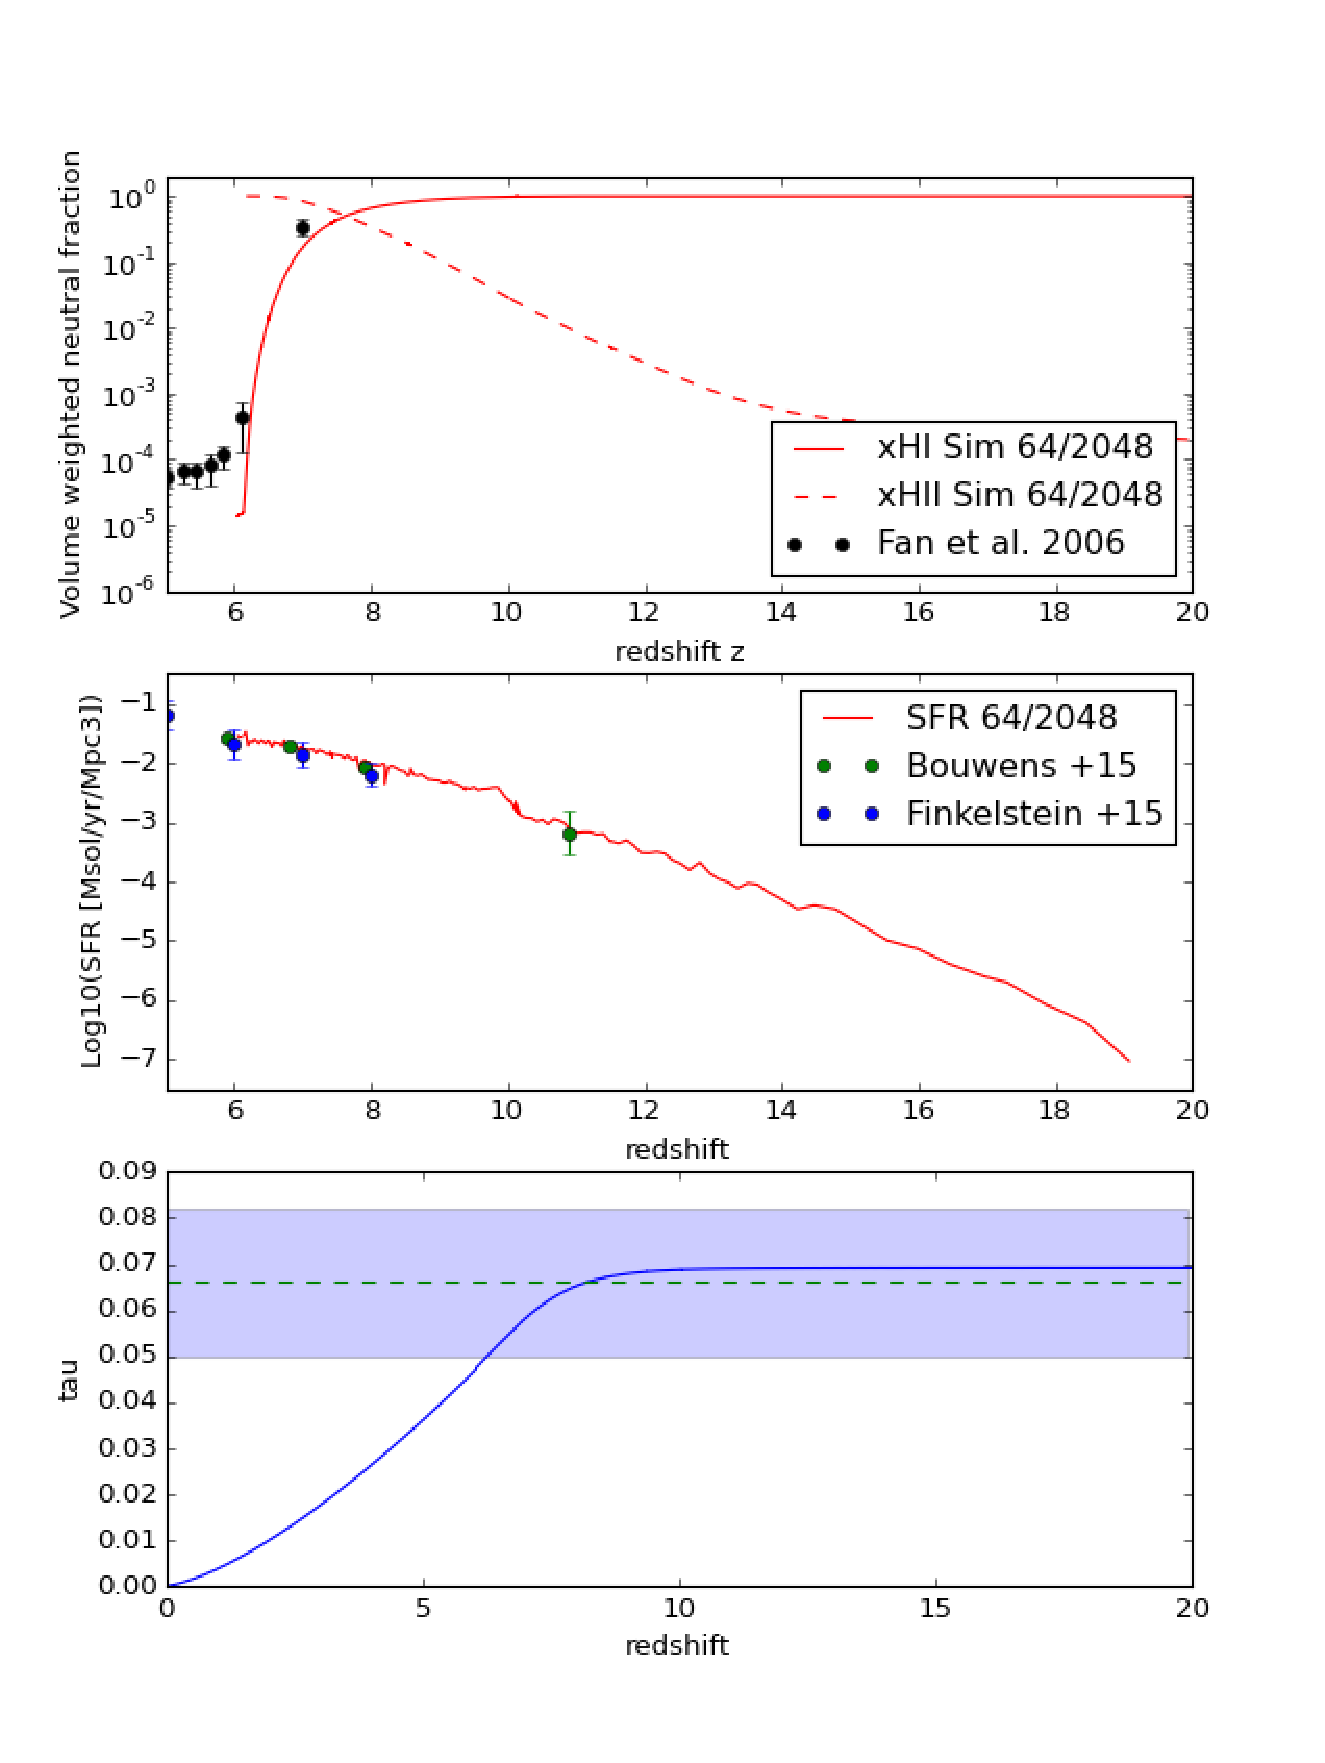
\includegraphics[width=.95\linewidth]{img/05/x_sfr_tau.pdf} 
        \caption[Contraintes CoDa I AMR]{ Variables globales de la simulation \ac{CoDa} I \ac{AMR} réalisée avec EMMA.
        Panneau supérieur : histoire d'ionisation
		Panneau central : SFH cosmique.
        Panneau inférieur : épaisseur optique Thomson.
        La simulation présente un bon accord avec les contraintes observationnelles.
		\label{fig:presCODAEMMA}}
\end{figure}


\section{Détermination des redshift de réionisation des halos à redshift z=0}

L'objectif est ici de créer le lien entre ces deux simulations en utilisant la carte de redshift d'ionisation d'un coté et la distribution de matière noire de l'autre.
L'idée est ici que le l'influence gravitationnelle des baryons est négligeable par rapport à celle de la matière noire.
Ce qui fait que l'introduction de l'hydrodynamique du gaz dans la simulation EMMA n'a pas significativement impacté la distribution de matière à redshift $z=6$ et que cette distribution est comparable à celle mesurée dans la simulation Gadget.
Cette hypothèse est vérifiée, dans une certaine mesure, sur la figure \ref{fig:zmapcomp}.
La population de halos trouvée dans la simulation Gadget est superposée à la carte de redshift de réionisation obtenue avec la simulation EMMA.
Les halos se trouvent effectivement aux centres des régions ionisées.
Il est donc a priori possible de lier la réionisation mesurée dans la simulation EMMA à l'évolution des structures mesurée dans la simulation Gadget.
La méthode de projection n'est pas unique est principalement deux pistes ont été explorées.
La figure \ref{fig:methodes} est une représentation graphique de ces deux méthodes.

%En considérant que le couplage entre la matière noire et les baryons et faible, la comparaison entre les catalogues de halos des deux simulations pris a la même époque peux être réalisé directement.

\begin{figure}
		\centering
        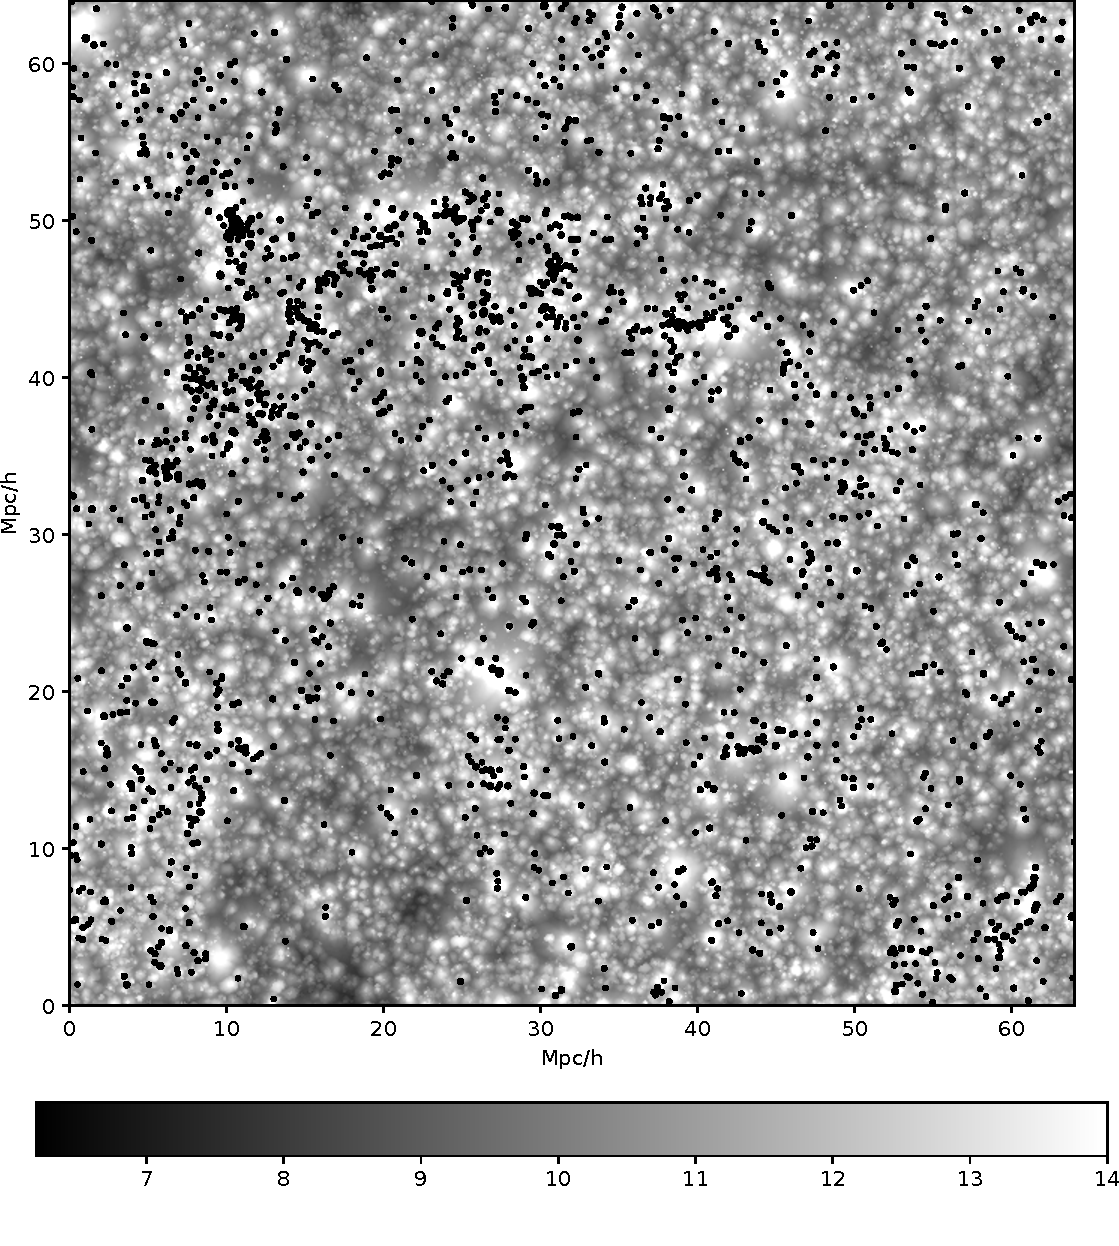
\includegraphics[width=.95\linewidth]{img/05/maphaloh.pdf} 
        \caption[Carte de redshift et halos]{Carte de redshift de reionisation calculée par la simulation \ac{RHD} et positions des halos à redsihft z=0 calculées avec la simulation, matière noire pure.
        La concordance des deux simulations est correcte, les halos de trouvent aux centre des régions ionisées.
		\label{fig:zmapcomp}}
\end{figure}

\clearpage

\begin{figure}
		\centering
        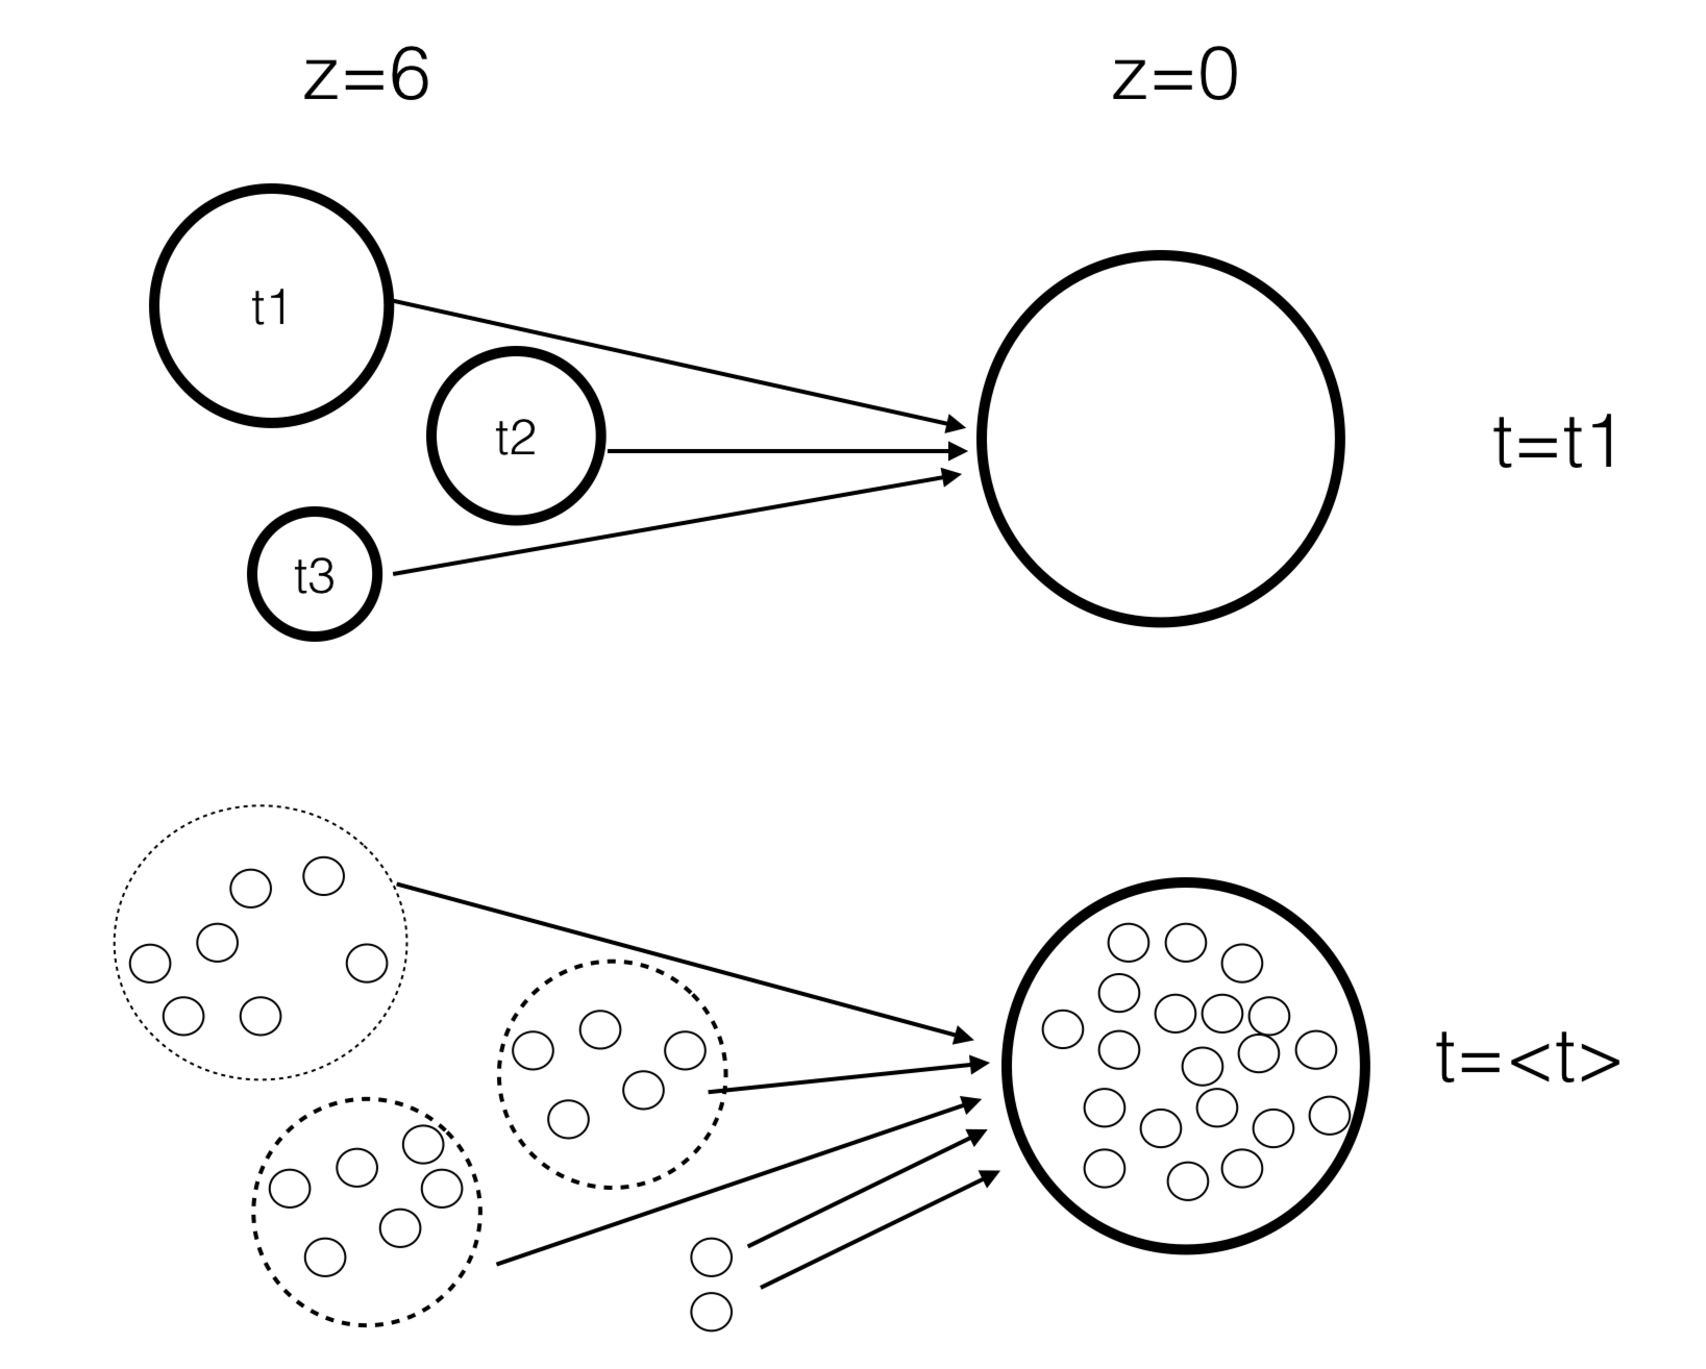
\includegraphics[width=.95\linewidth]{img/05/method.pdf} 
        \caption[Methodes]{Représentation des deux méthodes d'assignation de redshift de réionisation aux halos de la simulation gadget.
        Méthode "merger tree" en haut, méthode "particule" en bas
		\label{fig:methodes}}
\end{figure}


\subsection{Méthode "Merger Tree"}
La première méthode se base sur un un arbre de fusion (merger tree) des halos, généré sur la simulation Gadget.
%présentation du merger tree
Il permet de suivre les histoires de formation des halos de redshift $z=100$ jusqu'à nos jours.
En considérant un halo donné à redshift $z=0$, il est possible de déterminer, grâce a l'arbre de fusion, la position du centre de masse de tous ses halos progéniteurs à redshift $z=6$.
A chacune de ses position est ensuite associée un instant d'ionisation en utilisant la carte de redshift de réionisation.
Le redshift de réionisation associé au halo, et celui du progéniteur le plus massif à redshift $z=6$.
Cette méthode impose que le halo en question ait au moins un progéniteur à redshift $z=6$ et considère donc en priorité les halos les plus massifs.

\subsection{Méthode "Particules"}
La seconde technique utilise les positions de la totalité des particules de matière noire.
En ayant la liste de toutes les particules de matière noire d'un halo donné à redshift $z=0$, il est possible de retrouver leurs positions à redshift $z=6$.
De la même manière que précédemment, une liste de redshift de réionisation est obtenue pour chaque halo.
La valeur finale de redshift de réionisation associée au halo est la moyenne de cette liste.
Cette méthode permet de sonder les halos moins massifs qui n'avaient pas de progéniteurs redshift $z=6$, mais créer un effet de diffusion puisque des particules n'appartenant pas à des halos, et ayant des instants de réionisation plus tardif, se trouvent prisent en considération.

\section{Résultats}

Les résultats qui vont être présentés dans cette section représente une étude préliminaire globale de la simulation.
Évidemment, les simulations \ac{CoDa} ont encore énormément de potentiel scientifique à exploiter.

\subsection{Temps d'ionisation des halos}

Nous avons associé, pour chaque halos à redshift $z=0$ de la simulation Gadget, une liste de redshift de réionisation.
Il est donc possible de déterminer un redshift de réionisation moyen, ainsi qu'un temps de réionisation.
La figure \ref{fig:CODA_t} présente ces deux grandeurs.
Le panneau supérieur représente l'instant d'ionisation, en fonction de la masse du halo à $z=0$ pour les deux méthodes d'association.
Les traits représentent la valeur médiane dans l'intervalle de masses, les régions grisées représente limite de distributions à 5\% et 95\%.
On mesure ici que les halos les plus massifs reionises plus tôt indépendamment de la méthode.
Cependant la méthode du progéniteur a tendance a réioniser plus tôt, car elle se concentre sur les halo les plus massifs

Le second panneau de la figure \ref{fig:CODA_t} présente les durée necessaire à la réionisation des halos en fonction de leurs masses.
La méthode des particules a été utilisée, et pour chaque halo, une liste de redshift est associée.
\begin{itemize}
\item Dans un premier cas, la durée de réionisation a été associée à la différence entre l'instant où la première particule à été ionisé et l'instant où la dernière particule à été ionisée.
\item Dans le second cas, pour chaque halos, la distribution des redshift est approximée par une distribution normale, et la durée associée est l'écart à 2$\sigma$ de cette distribution.
Cette méthode limite les durées extrêmes et en moyenne la durée est toujours plus basse que dans la première méthode.
\end{itemize}

Dans les deux méthodes, les halos les plus massifs ont une durée de réionisation plus importante. 
Pour les halos les moins massifs ($M<10^9 M_\odot$)

\begin{figure}
		\centering
        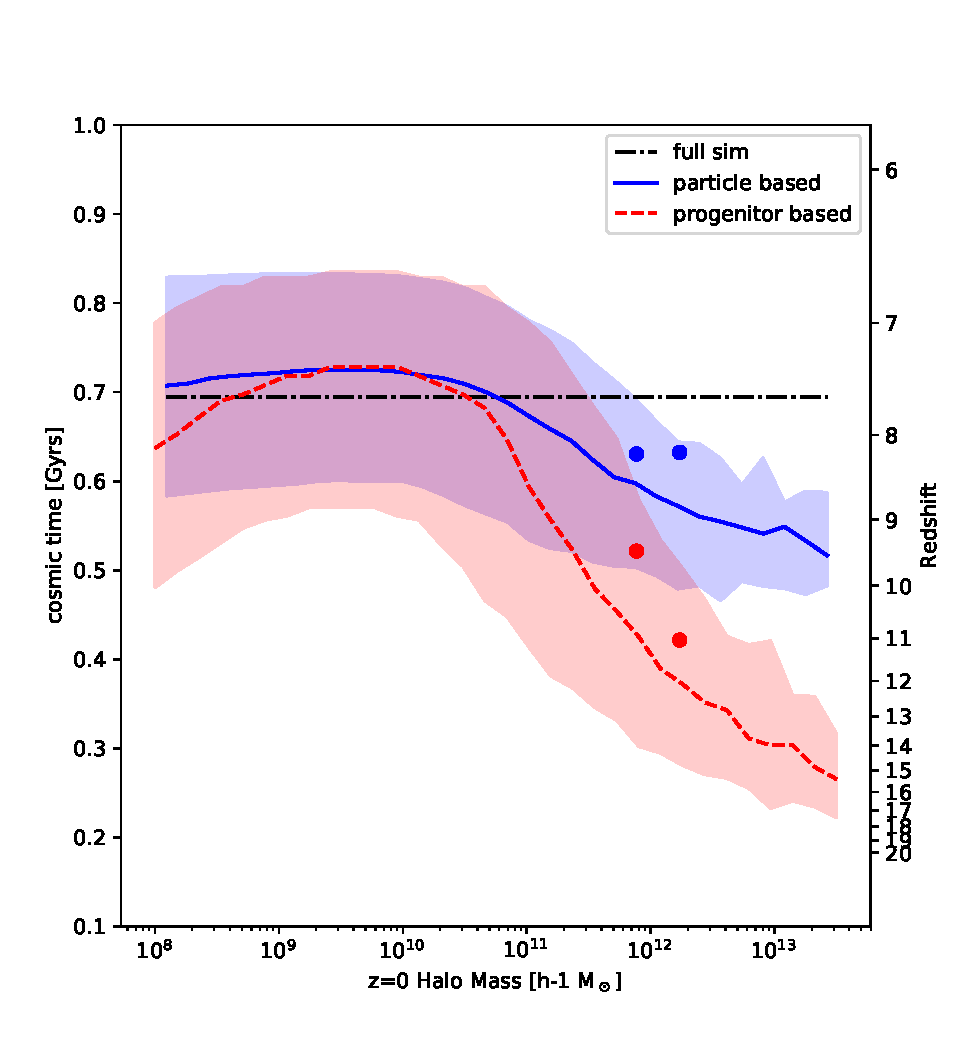
\includegraphics[width=.95\linewidth]{img/05/track_treion_LG.pdf}
        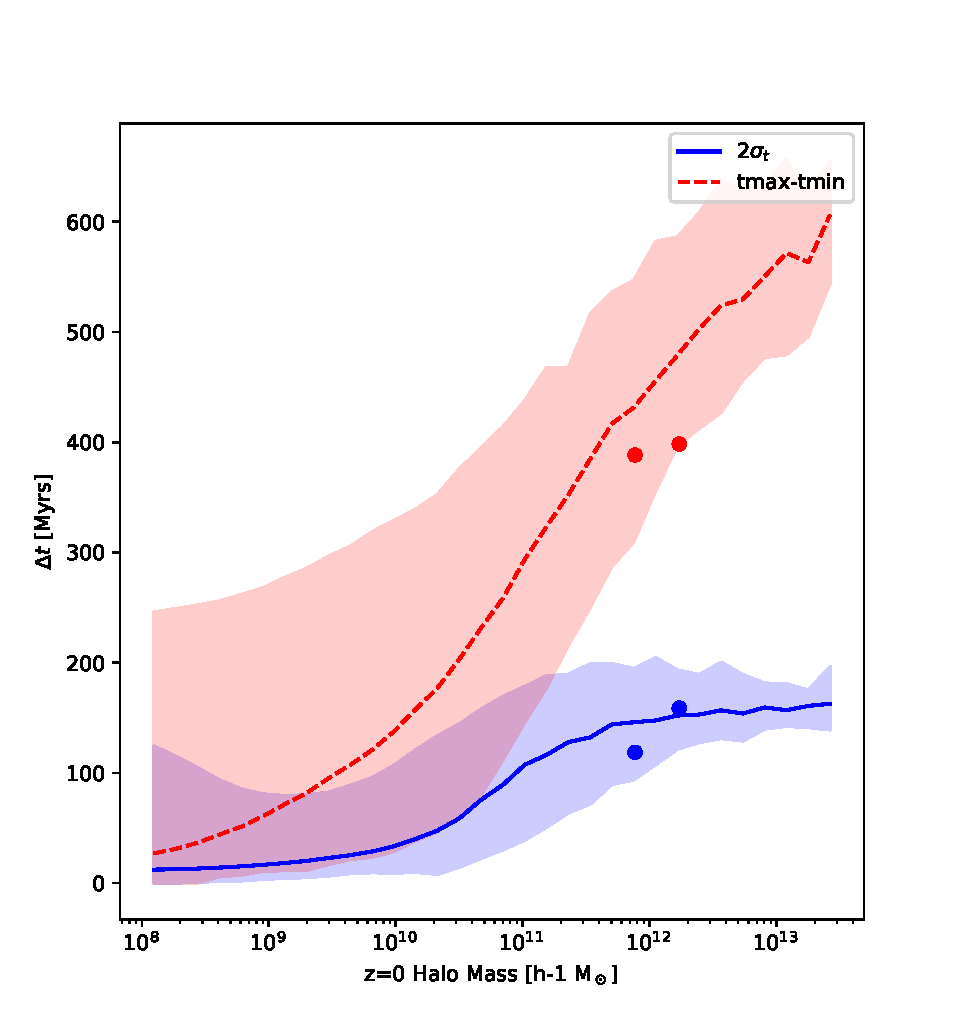
\includegraphics[width=.95\linewidth]{img/05/track_dt_2sig_LG.pdf} 
        \caption[t et dt reio]{
		\label{fig:CODA_t}}
\end{figure}

\clearpage
\subsection{Étude d’environnement}

Le volume total de la simulation a été découpé en parties égales.
A cause de la variance cosmique, chacune de ses sous partie dispose de sa propre densité moyenne
La figure \ref{fig:CODA_environnement} présent la comparaison des durées de réionisation obtenues avec la méthode 2$\sigma$, sur l'ensemble du volume, dans le sous volume le moins dense et dans le sous volume le plus dense.
Nous mesurons, qu'un environnement dense mène en moyenne à une durée de réionisation plus courte.

\begin{figure}
		\centering
		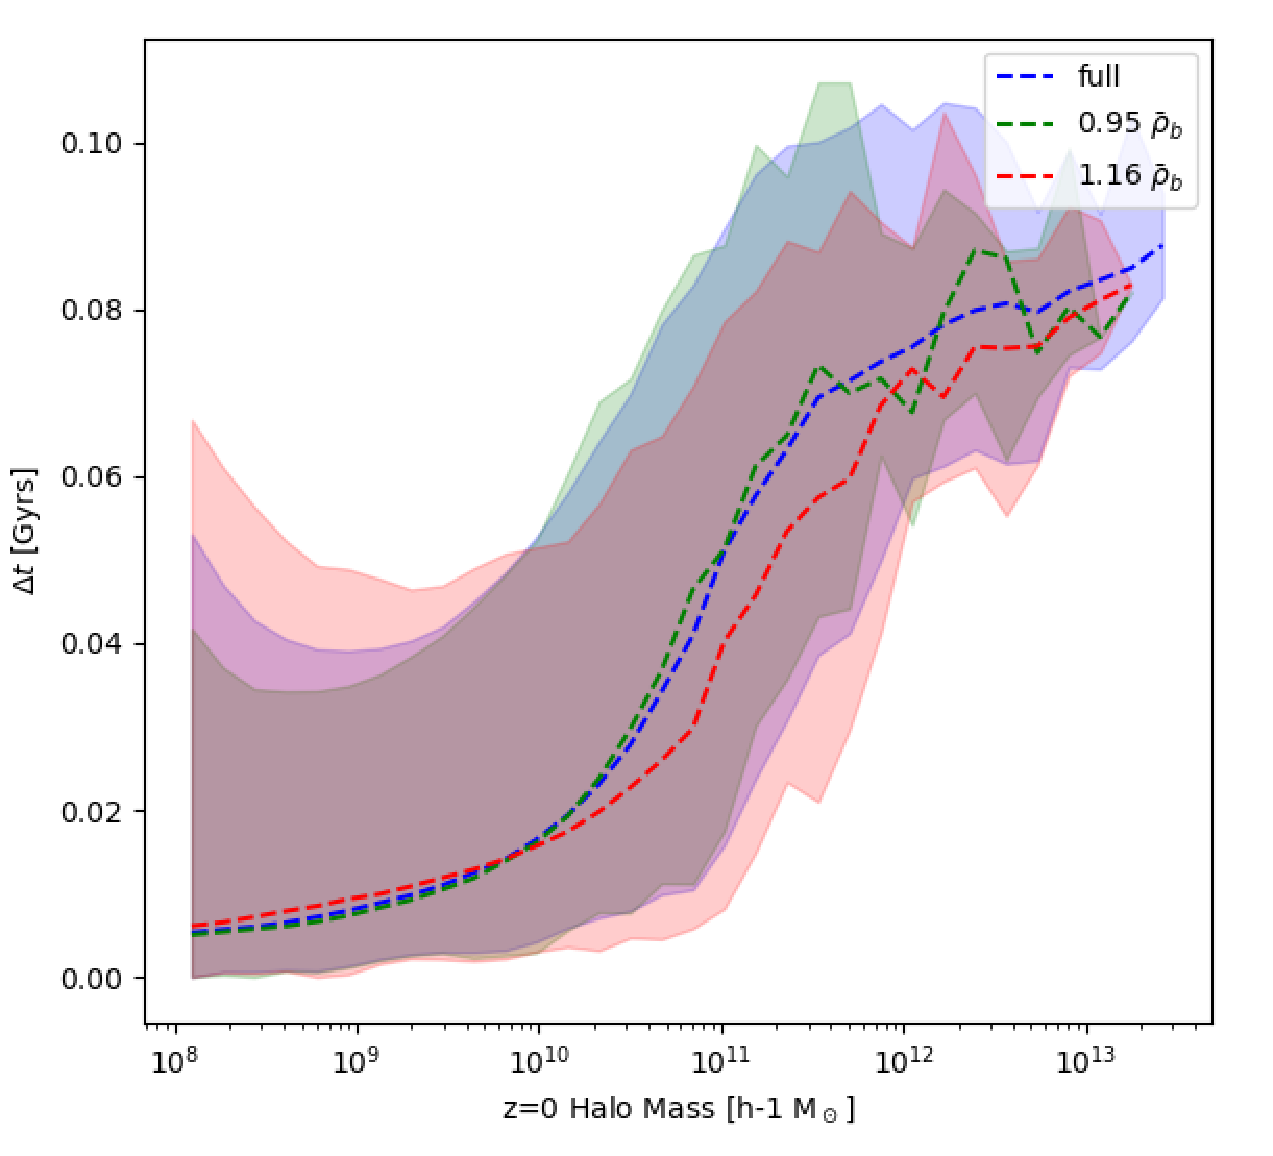
\includegraphics[width=.95\linewidth]{img/05/median_dt_envir.pdf}
        \caption[influence de l'environement]{
		\label{fig:CODA_environnement}}
\end{figure}

\subsection{Le cas du groupe local}
\begin{figure}
		\centering
		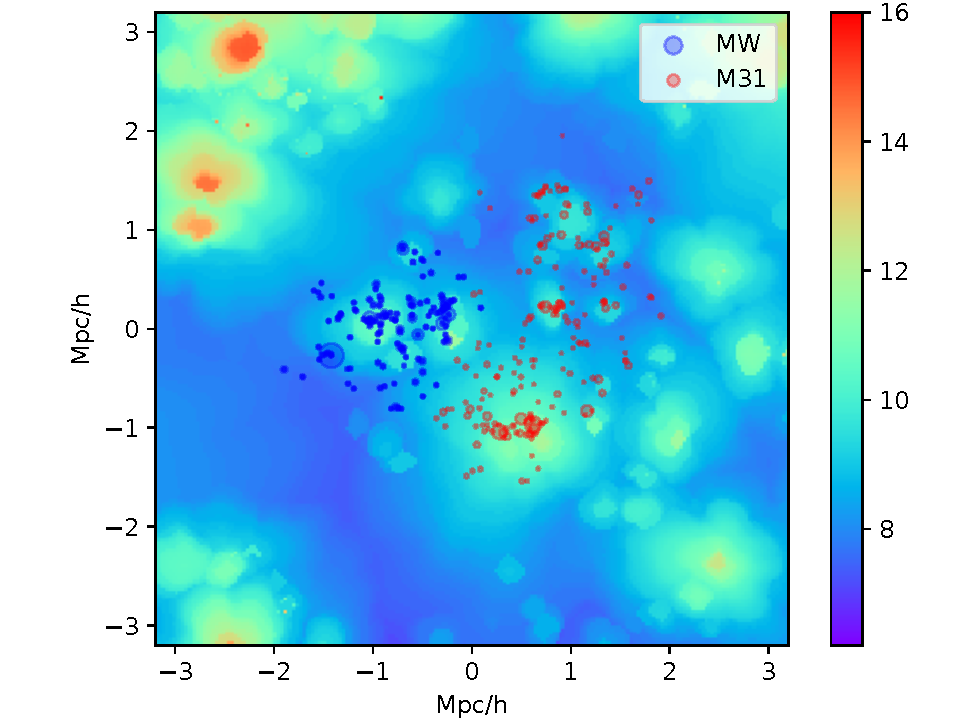
\includegraphics[width=.95\linewidth]{img/05/map_LG.pdf}
        \caption[Groupe local]{
		\label{fig:CODA_LG}}
\end{figure}

